\documentclass{article}
\usepackage[utf8]{inputenc}

\usepackage{tikz}
\usetikzlibrary{positioning}

\begin{document}

\begin{figure}
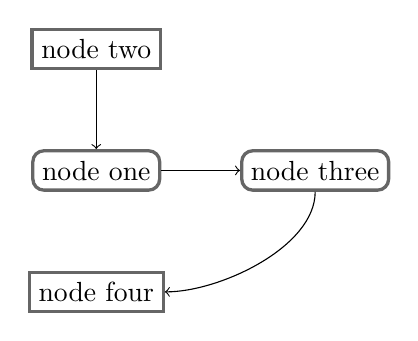
\begin{tikzpicture}[ % has a lot of options; consult the manual
square/.style={rectangle, draw=black!60, very thick, minimum size=5mm},
square_rounded/.style={rectangle, rounded corners, draw=black!60, very thick, minimum size=5mm},
]

% \node[type](name_of_node)[above/below/right/left/...=of name_of_node]{text_in_node}
\node[square_rounded](maintopic){node one};
\node[square](uppercircle)[above=of maintopic]{node two};
\node[square_rounded](rightsquare)[right=of maintopic]{node three};
\node[square](lowercircle)[below=of maintopic]{node four};

% \draw[->] (name_of_node.direction) -- (name_of_node.direction)
\draw[->] (uppercircle.south) -- (maintopic.north);
\draw[->] (maintopic.east) -- (rightsquare.west);
\draw[->] (rightsquare.south) .. controls +(down:7mm) and +(right:7mm) .. (lowercircle.east);

\end{tikzpicture}
\end{figure}

\end{document}